\begin{center}
    \section*{\fontsize{20}{20}\selectfont Chapter 5}
\end{center}
\vspace{10mm}

\section{Standards, Constraints, and Milestones}

While the technical implementation and performance metrics discussed in the previous chapters demonstrate the feasibility of the proposed plant disease detection system, it is equally important to evaluate the system through the lens of engineering standards, societal impact, and ethical considerations. This chapter outlines the compliance with industry standards adopted during development, analyzes the potential impact of this technology on agriculture and society, and discusses the ethical responsibilities associated with deploying AI in real-world scenarios. Furthermore, it highlights the technical challenges faced during the research and the constraints that define the scope of this work.

\subsection{Sustainability Standards}
To ensure the reliability, maintainability, and reproducibility of the research, strictly defined engineering and software standards were adhered to throughout the development lifecycle:
\begin{itemize}
    \item \textbf{Software Coding Standards (PEP 8):} The entire codebase was written in Python adhering to the PEP 8 style guide. This ensured consistent indentation, naming conventions (e.g., \texttt{snake\_case} for functions, \texttt{CamelCase} for classes), and code readability, making the project open-source friendly.
    \item \textbf{Data Licensing Standards:} The dataset was obtained from a public Kaggle repository and is used only for educational and research purposes, following the license terms of its authors.
    \item \textbf{Model Evaluation Standards:} Standard evaluation metrics defined by the machine learning community---Accuracy, Precision, Recall, F1-Score, and Confusion Matrix---were used to validate the models, ensuring the results are comparable with existing literature.
\end{itemize}

\subsection{Impacts on Society}
The deployment of an automated plant disease detection system has far-reaching implications for society, particularly in the agricultural sector:
\begin{itemize}
    \item \textbf{Food Security:} Early detection of potato problems such as Phytopthora (late blight), fungal and bacterial diseases, viruses and pests can help prevent large crop losses. This supports Sustainable Development Goal (SDG) 2: Zero Hunger.
    \item \textbf{Economic Benefits for Farmers:} In many developing regions, farmers rely on expensive agricultural experts or on guesswork that can lead to crop failure. Once the system reaches a reliable accuracy, it can provide a low-cost first-level diagnosis and simple advice through the LLM module, which reduces costs and prevents losses.
    \item \textbf{Environmental Sustainability:} Misdiagnosis often leads to the excessive and indiscriminate use of pesticides. By accurately identifying the specific disease, farmers can apply targeted treatments (precision agriculture), thereby reducing chemical runoff into soil and water, which protects the ecosystem.
\end{itemize}

\subsection{Ethics}
Deploying Artificial Intelligence in agriculture brings specific ethical responsibilities that have been addressed in this research:
\begin{itemize}
    \item \textbf{Algorithmic Bias:} The dataset has a class imbalance (748 Fungi images vs.\ 68 Nematode images). The results show that this bias is real, because two models predicted only one class. To reduce this risk, stratified splitting and data augmentation were used, and class weighting is planned for future training.
    \item \textbf{Risk of Misdiagnosis (False Negatives):} Telling a farmer that a diseased plant is healthy, or giving the wrong disease, can cause crop loss. Label smoothing was used to reduce overconfidence, and the LLM is instructed to warn the user when the confidence is low. The current models must not be used for real decisions until they reach a validated accuracy.
    \item \textbf{Data Privacy and Responsible LLM Use:} The dataset does not contain personal data. The Gemini API key is stored in Kaggle Secrets, not in the code. Only the predicted class and the confidence are sent to the LLM (not the image), and the prompt forbids invented pesticide doses.
\end{itemize}

\subsection{Challenges}
During the research and implementation phase, several significant challenges were encountered and addressed:
\begin{itemize}
    \item \textbf{Severe Class Imbalance:} The dataset is skewed (about 11:1). Training on this data led the models to favor majority classes (Pest and Fungi). Stratified splitting and augmentation were used, but stronger methods such as class weights or oversampling are still needed.
    \item \textbf{Complex Field Backgrounds and Similar Symptoms:} The images contain soil, hands, plastic mulch and other plants, and different problems (for example, Fungi and Phytopthora) can show similar brown lesions. This makes the task much harder than with laboratory datasets.
    \item \textbf{Hardware Limitations:} In the reported run, the GPU could not be initialized, so all models were trained on the CPU (about 4 to 9 minutes per epoch). This limited the training to 6 to 10 epochs. In addition, ImageNet weights were not downloaded, so ResNet50 and MobileNetV2 could not use transfer learning.
\end{itemize}

\subsection{Constraints}
Every research project operates within certain boundaries. The limitations of this work are outlined below:
\begin{itemize}
    \item \textbf{Dataset Scope:} The system is limited to the 7 classes of the potato dataset. It cannot detect diseases of other crops (for example, rice or wheat).
    \item \textbf{Small Dataset Size:} With 3,076 images (and only 68 Nematode images), the dataset is small for training deep networks from scratch.
    \item \textbf{Computational Resources:} Training was limited to 15 epochs for the Custom CNN and 10 epochs for the benchmark models at $224 \times 224$ resolution, and it ran on the CPU.
    \item \textbf{Connectivity:} The LLM advisory module needs an internet connection to call the Gemini API, which can be a constraint in remote rural areas.
\end{itemize}

\subsection{Timeline and Gantt Chart}
To ensure the successful completion of this research within the stipulated timeframe of six months, a structured work schedule was established. The project lifecycle was divided into two primary phases: Phase I (Planning and Design) and Phase II (Implementation and Analysis). The breakdown of tasks and their respective timelines are visualized using Gantt charts in Figure~\ref{fig:gantt1} and Figure~\ref{fig:gantt2}.

\subsubsection{Phase I: Planning and System Design (Weeks 1--13)}
The first phase focused on laying the theoretical foundation and preparing the necessary resources for the experiment. As illustrated in Figure~\ref{fig:gantt1}, this phase spanned the first three months (Weeks 1 to 13):
\begin{itemize}
    \item \textbf{Weeks 1--2:} Comprehensive literature review to identify gaps in existing plant disease detection methods.
    \item \textbf{Weeks 3--5:} Collection of the Potato Leaf Disease (Uncontrolled Environment) dataset, followed by Exploratory Data Analysis (EDA) to understand the class distributions.
    \item \textbf{Weeks 6--10:} Designing the architecture of the proposed Custom Lightweight CNN and setting up the preprocessing pipelines (normalization, augmentation).
    \item \textbf{Weeks 11--13:} Selecting and configuring transfer learning models (ResNet50, MobileNetV2) and finalizing the research methodology.
\end{itemize}

\begin{figure}[htbp]
\centering
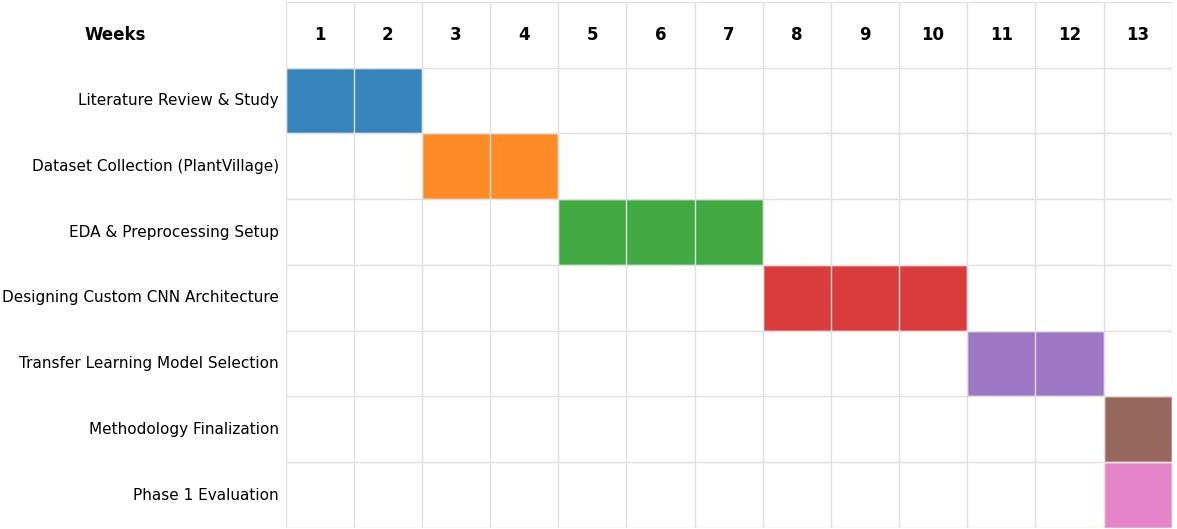
\includegraphics[width=0.95\textwidth]{image/docx_image26.jpeg}
\caption{Gantt Chart I -- Timeline for Planning, Data Preparation, and Model Design (Weeks 1--13).}
\label{fig:gantt1}
\end{figure}

\subsubsection{Phase II: Implementation, Testing, and Documentation (Weeks 14--26)}
The second phase was dedicated to the practical execution, rigorous testing, and documentation of the research findings. As depicted in Figure~\ref{fig:gantt2}, this phase covered the remaining three months (Weeks 14 to 26):
\begin{itemize}
    \item \textbf{Weeks 14--17:} Training the three models (Custom CNN, ResNet50, MobileNetV2) and performing hyperparameter tuning to optimize accuracy.
    \item \textbf{Weeks 18--21:} Conducting a comparative analysis of the models based on accuracy, loss and inference speed. In addition, Explainable AI (Grad-CAM) and the Gemini-based LLM advisory module were implemented during this period.
    \item \textbf{Weeks 22--26:} Finalizing the results, visualizing performance metrics (Confusion Matrix, ROC Curves), and compiling the complete thesis report. The phase concluded with the preparation for the final defense presentation.
\end{itemize}

\begin{figure}[htbp]
\centering
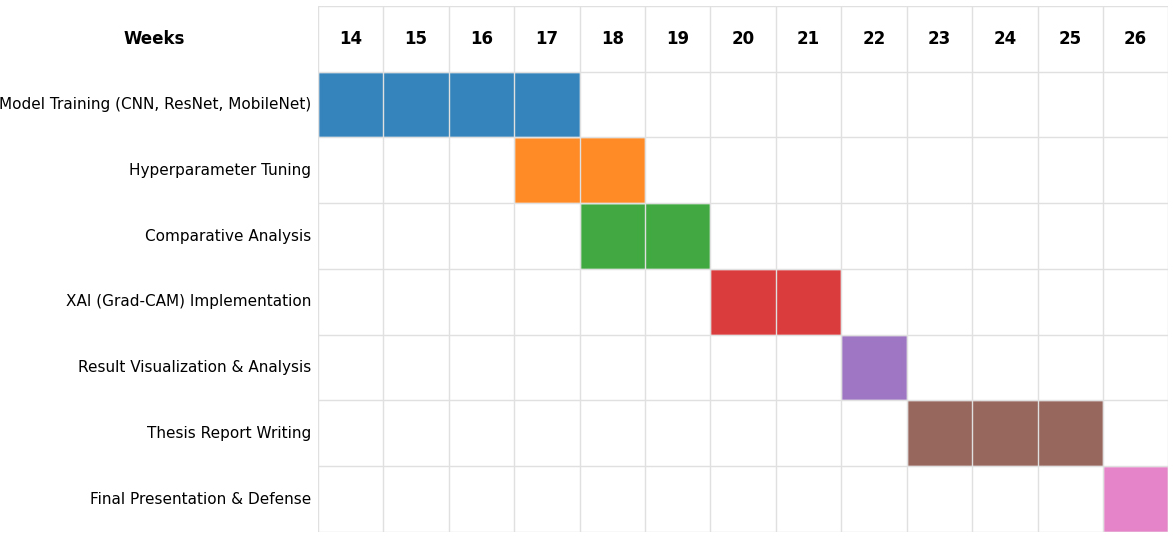
\includegraphics[width=0.95\textwidth]{image/docx_image27.png}
\caption{Gantt Chart II -- Timeline for Implementation, Testing, and Final Documentation (Weeks 14--26).}
\label{fig:gantt2}
\end{figure}

\subsection*{Summary}
This chapter discussed the non-technical dimensions of the research. The project follows coding and data standards. The societal impact analysis showed the potential of the system for food security and environmental sustainability. Ethical issues such as class bias, misdiagnosis and responsible LLM use were addressed. Finally, the challenges of class imbalance, complex backgrounds and limited hardware, and the constraints of dataset size and connectivity, were described to give a realistic view of the current system.
